\chapter{Interfaz Hardware - Software}
\par La interfaz de comunicación entre la estación de recolección y el Software (Aplicación) debe permitir transmitir los datos obtenidos recolectados por la primera hacia la Aplicación de manera confiable. La Aplicación, por su parte, es la encargada de procesar los datos y enviar las señales correspondientes de vuelta al Raspberry\textsuperscript{\textregistered}.

    \section{Análisis de alternativas}
        \subsection{Alternativas}
            \subsubsection{Tecnologías alámbricas}
                \par Esta opción se desestima para ser utilizada de este proyecto por una decisión del diseño planteado en el anteproyecto.
            \subsubsection{Tecnologías inalámbricas}
                \par Dentro de esta tecnología se encuentran los estándares más utilizados: Wi-Fi\textsuperscript{\textregistered} (IEEE\footnote{ \textit{Institute of Electrical and Electronics Engineers}, Instituto de Ingeniería Eléctrica y Electrónica} 802.11x) y Bluetooth\textsuperscript{\textregistered} (IEEE 802.15x).
                
                \paragraph{Wi-Fi\textsuperscript{\textregistered}:} Es una marca comercial de Wi-Fi Alliance (una organización que adopta y certifica los equipos que cumplen con los estándares 802.11 de las redes inalámbricas de área local). El objetivo tras la marca Wi-Fi\textsuperscript{\textregistered} es fomentar las conexiones inalámbricas y facilitar la compatibilidad de los distintos equipos.
                
                \par Esta tecnología permite la comunicación de datos entre un dispositivo y todos aquellos que se encuentren dentro del área de cobertura del mismo o de la red de un punto de acceso al que se encuentre conectado este. Para ello utiliza enlace de radio frecuencia de 2.4, 3.6 o 5Ghz, dependiendo el estándar que se utilice.
                
                \paragraph{Bluetooth\textsuperscript{\textregistered}:} Bluetooth\textsuperscript{\textregistered} es una especificación industrial para Redes Inalámbricas de Área Personal (WPAN) creado por Bluetooth Special Interest Group, Inc. que posibilita la transmisión de voz y datos entre diferentes dispositivos mediante un enlace por radiofrecuencia en la banda ISM de los 2.4 GHz.
                
        \subsection{Comparación}
            \par A continuación se presenta una tabla comparativa de ambas tecnologías. Se utilizarán como criterios de comparación aquellos relevantes para la realización del proyecto:
            
            \begin{table}[h]
                \centering
                \begin{tabularx}{\textwidth}{|X|X|X|}
                    \hline
                    \multicolumn{3}{|c|}{\textbf{Comparación de tecnologías inalámbricas}}
                    \\
                     \hline
                      & Bluetooth\textsuperscript{\textregistered} & Wi-Fi\textsuperscript{\textregistered}  \\ \hline \hline
                     
                     Frecuencia & 2.4 GHz & 2.4, 3.6, 5 GHz \\ \hline 
                     
                     Ancho de banda (Bandwidth) & Bajo (800 kbps) & Alto (11 Mbps en 802.11b) \\ \hline
                     
                     Autoridad de especificación & Bluetooth SIG\footnote{ Bluetooth Special Interest Group, asociación privada sin ánimo de lucro} & IEEE, WECA \\ \hline
                     
                     Seguridad & Poco seguro & Más seguro \\ \hline
                     
                     Dispositivos principales & Teléfonos inteligentes, ratones, teclados, etc & Notebook, Computadoras de escritorio, Servidores, TV, Teléfonos inteligentes, etc\\ \hline
                     
                     Requerimientos de Hardware & Adaptador Bluetooth en todos los dispositivos & Adaptadores inalámbricos (Wireless) en todos los dispositivos de la red, wireless router y/o wireless access point \\ \hline
                    
                     Cantidad de dispositivos conectados & Solo dos & Múltiples\\ \hline
                     
                     Rango & 5-30 metros & 32-300 metros \\ \hline
                     
                     Consumo de Energía & Bajo & Alto \\ \hline
                     
                     Latencia & 200 ms & 150 ms \\ \hline
                     
                     Tasa de transferencia (Bit-rate) & 2.1 Mbps & 600 Mbps\\ \hline
                \end{tabularx}
                \caption{Comparación de tecnologías inalámbricas Bluetooth\textsuperscript{\textregistered} y Wi-Fi\textsuperscript{\textregistered}}
                \label{tab:ComparacionInterfaz}
            \end{table}
        \subsection{Tecnologías utilizadas}
            A partir de los datos comparados de la Tabla \ref{tab:ComparacionInterfaz}, se opta por utilizar la tecnología WiFi, dadas sus características de seguridad, rango y cantidad de dispositivos conectados, satisfaciendo con esta los objetivos de este proyecto.
            A partir de la elección del protocolo de comunicación inalámbrica, se define construir un servidor web que opere sobre el componente electrónico, y en forma posterior, un servicio web REST API \footnote{REST API, representational state transfer (REST) application program interface (API), es una interfaz que utiliza requerimientos HTTP tipo GET, PUT, POST and DELETE para transferencia de datos.}, funcionando en este contexto, que permita establecer una comunicación entre el dispositivo móvil y el componente electrónico.
            Dadas las recomendaciones del fabricante del componente electrónico, la multiplicidad de guías, comunidad y soporte, se opta por la utilización de la tecnología Apache para la construcción del servidor web. A partir de esta elección se propone PHP\footnote{PHP (acrónimo recursivo de PHP: Hypertext Preprocessor) es un lenguaje de código abierto muy popular especialmente adecuado para el desarrollo web.} como tecnología de desarrollo, por cuestiones de agilidad y coexistencia.

    
    \section{Diseño}
        
        \subsection{Consideraciones Previas}
            \par En este apartado se describen distintas restricciones inherentes al funcionamiento del sistema que se consideraron para el diseño del mismo. Cada una será descrita con el fin de fundamentar la decisión de diseño elegida.

            \paragraph{Capacidad de ejecutar código Python:}
                \par Los scripts para obtención y almacenamiento de mediciones fueron escritos en lenguaje Python. Por esto, la API REST debe poder ejecutar este tipo de archivos. Las llamadas de ejecución deben permitir adjuntar parámetros de configuración.
        
            \paragraph{Capacidad de establecer conexión con la base de datos:} 
                \par La REST API debe poder conectarse a la base de datos alojada en el servidor para realizar lectura y escritura de datos.
        
            \paragraph{Capacidad de ejecutar distintas funcionalidades en forma paralela:}
                \par Es requisito del sistema ejecutar de manera simultánea y continua la transmisión de datos entre el componente de hardware y software mientras se procede con la recolección de datos de la experiencia.
        
            \paragraph{Capacidad de mantener la coherencia de datos:}
                \par La detección de una falla durante el experimento es detectado por el componente de software. Por ende, la interfaz debe ofrecer la posibilidad de eliminar los datos corruptos correspondientes a una maceración inconclusa de la base de datos alojada en el componente electrónico con el fin de mantener la coherencia de los datos.
                
        
        \subsection{Diseño de la interfaz}
        \begin{minipage}{0.95\textwidth}
            \par En cuanto al diseño de la REST API, se opta por codificar cada funcionalidad en un archivo independiente y cumplir de esta manera con la consideración previa de ejecución paralela.
            \par A continuación (Tabla \ref{tab:FuncionalidadesInterfaz}), se presenta una descripción de funcionalidades:
            \\
            \end{minipage}
        \begin{minipage}{\textwidth}
            
                \centering
                \begin{tabularx}{\textwidth}{|X|X|X|X|}
                    \hline
                    \multicolumn{4}{|c|}{\textbf{Funcionalidades de la Interfaz}} \\
                    \hline
                    Nombre & Funcionalidad & Retorno & Parámetros \\ 
                    \hline 
                    \hline
                    
                    Inicio de Experiencia de Maceración & Inserta en la base de datos la maceración, en caso de ser una nueva entrada, y el experimento. Ejecuta los archivos Python utilizando como parámetros la duración del experimento y los intervalos de medición & & Nombre maceración,  duración, intervalos de medición de temperatura y pH, e ID de Experimento \\ 
                    \hline
                    Obtención de valores recolectados de un experimento de Maceración & A partir de un ID de experimento y una lista de valores recolectados (obtenidos previamente por la aplicación), la API REST consulta la base de datos y retorna las mediciones correspondientes a cada ID de experimento no presente en el conjunto enviado & Arreglo de medidas por experimento. N conjuntos de: Medidas de temperatura del líquido; pH; temperatura y humedad ambiente & ID experimento, Lista de valores recolectados obtenidos en consultas anteriores \\ 
                    \hline
                    
              
                \end{tabularx}
                \captionof{table}{Descripción de funcionalidades de la interfaz Hardware-Software}
                \label{tab:FuncionalidadesInterfaz}
            
            \end{minipage}
            
            \begin{table}[H]
                \centering
                \begin{tabularx}{\textwidth}{|X|X|X|X|}
                    \hline
                    \multicolumn{4}{|c|}{\textbf{Funcionalidades de la Interfaz cont.}} \\
                    \hline
                    Nombre & Funcionalidad & Retorno & Parámetros \\ \hline \hline
                    
                    Obtención de datos de sensores & 
                    El componente de software (previsto a desarrollarse en las siguientes etapas) permite visualizar los valores actuales de los sensores. La funcionalidad encargada de acción ejecuta una rutina python y retorna los valores a través de la API REST. & Medidas de temperatura del líquido; pH; temperatura y humedad ambiente & \\
                    \hline
                    
                    Eliminación de un experimento de maceración & Eliminar el experimento y todos los datos recolectados que posean el ID de experimento pasado como parámetro &  & ID experimento\\
                    \hline
                    
                    Cancelación de un experimento de maceración & Detiene la ejecución de la librería Python, elimina los valores recolectados relacionados al ID de experimento y finalmente elimina el experimento mismo. & & ID experimento
                    \\
                    \hline
                    
                \end{tabularx}
                \caption{Descripción de funcionalidades de la interfaz Hardware-Software}
                \label{tab:FuncionalidadesInterfazCont}
            \end{table}

    \section{Implementación del componente}
        \par En esta sección se describe el funcionamiento de la API REST desarrollada mediante diagramas de flujo de cada funcionalidad.
        
        \subsection{Inicio de experimento de maceración}
        \par A continuación, (Figura \ref{fig:ApiNuevoExp}), se presenta el diagrama correspondiente a la API ``\textit{NuevoExp.php}'', la misma, realiza la inserción de una nueva maceración y de un experimento, luego, inicia el proceso de recolección de datos.
            \begin{figure} [h]
                \centering
                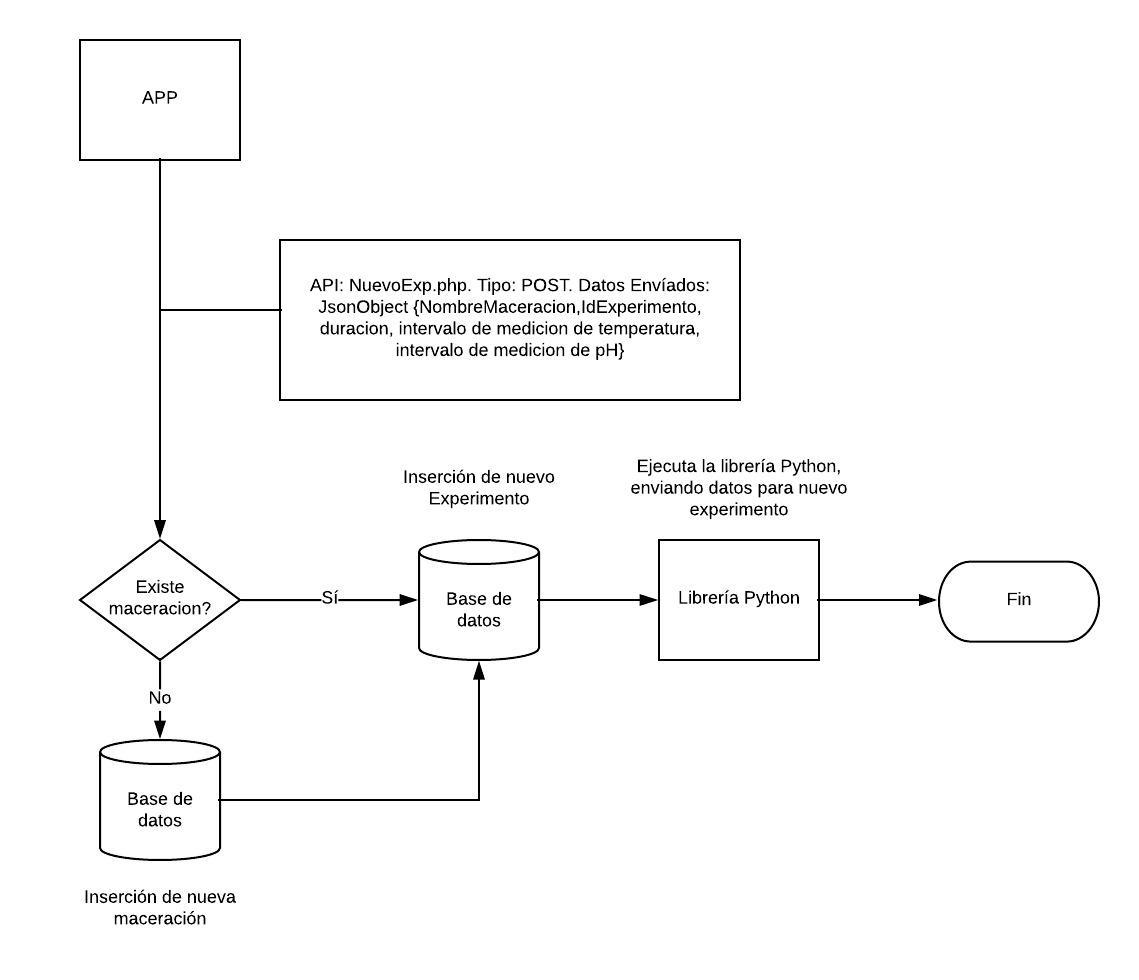
\includegraphics[scale=0.85]{DiagramaNuevoExp.jpeg}
                \caption{Diagrama de flujo para nuevo experimento}
                \label{fig:ApiNuevoExp}
            \end{figure}
            
        \subsection{Obtención de valores recolectados de un experimento de maceración}
        \par En la Figura \ref{fig:ApiGet}, se presenta el diagrama correspondiente a la API ``\textit{ObtenerSensedValues.php}'', la misma es responsable de la obtención de de nuevos conjuntos de valores recolectados relacionados a un Id de Experimento particular, y su posterior envío a la aplicación móvil.
            \begin{figure} [htb]
                \centering
                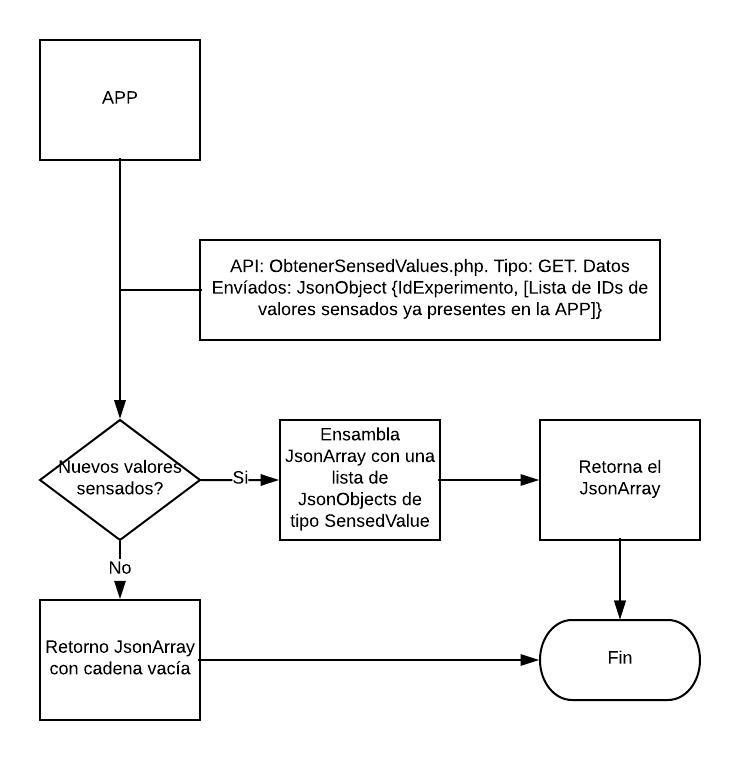
\includegraphics{DiagramaAPIGet.jpeg}
                \caption{Diagrama de flujo obtención de valores sensados}
                \label{fig:ApiGet}
            \end{figure}
        
        \subsection{Obtención de datos de sensores}
        \par La API ``\textit{ObtenerMediciónActual.php}'', es responsable de la obtención de de nuevos conjuntos de valores recolectados relacionados a un Id de Experimento particular, y su posterior envío a la aplicación móvil. El diagrama de la misma se visualiza en la Figura \ref{fig:ApiGetTempPh}
        
            \begin{figure}[htb]
                \centering
                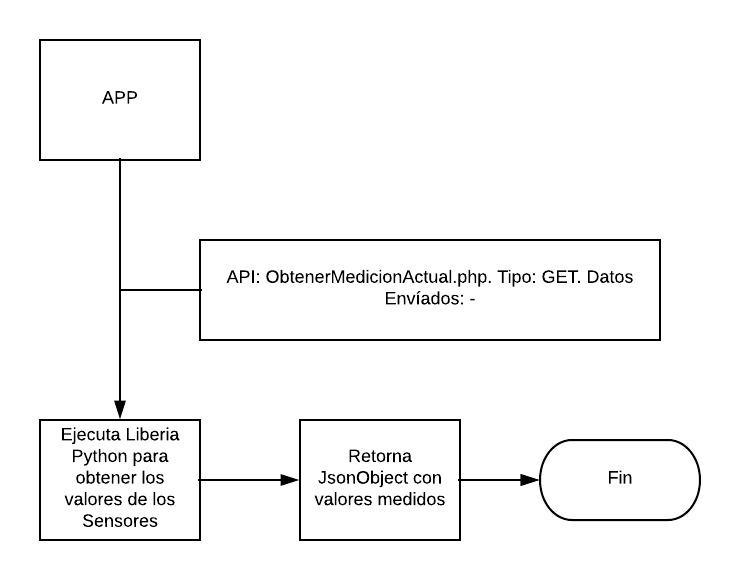
\includegraphics{DiagramaGetTempPh.jpeg}
                \caption{Diagrama de flujo de obtención de datos de sensores}
                \label{fig:ApiGetTempPh}
            \end{figure}
        
        \subsection{Eliminación experimento de maceración}
        \par A continuación, (Figura \ref{fig:ApiRemoveExp}), se presenta el diagrama correspondiente a la API ``\textit{EliminarExp.php}'', la misma, es responsable de la eliminación de un Experimento en la base de datos de la estación de recolección.
            \begin{figure} [htb]
                \centering
                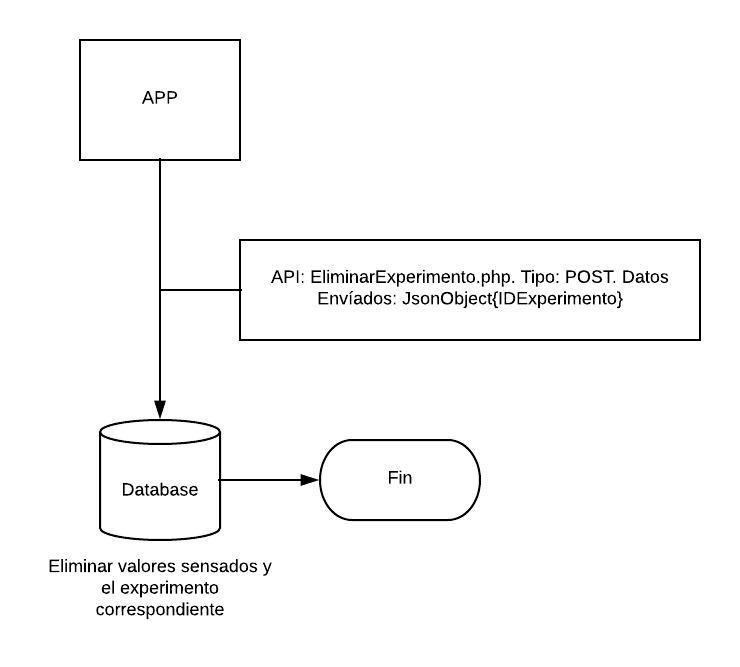
\includegraphics{DiagramaRemoveExp.jpeg}
                \caption{Diagrama de flujo de eliminación de experimento}
                \label{fig:ApiRemoveExp}
            \end{figure}
            
        \subsection{Cancelación experimento de maceración}
            \par En la Figura \ref{fig:ApiCancelExp} se presenta el diagrama correspondiente a la API ``\textit{CancelarExp.php}'', la misma, es responsable de la cancelación y eliminación de un experimento mientras el mismo se esta llevando a cabo.
            \begin{figure}[htb]
                \centering
                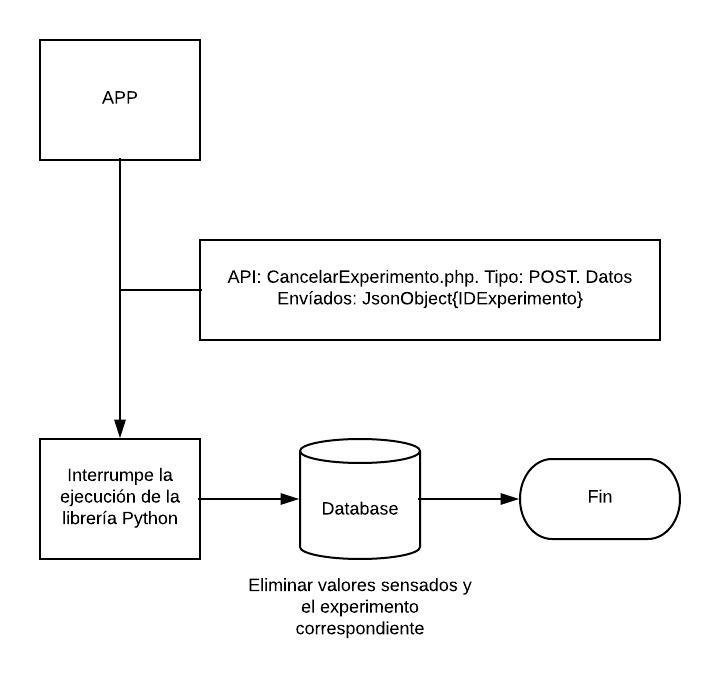
\includegraphics{DiagramaCancelExp.jpeg}
                \caption{Diagrama de flujo de cancelación de experimento en curso}
                \label{fig:ApiCancelExp}
            \end{figure}
        